\documentclass[12pt]{article}

\usepackage[utf8]{inputenc}
\usepackage[english]{babel}
\usepackage{fancyhdr}
\usepackage{graphicx}
\graphicspath{ {./images/} }
\usepackage{titling}
\usepackage{wrapfig}
\usepackage{float}
\usepackage[table,xcdraw]{xcolor}
\usepackage{blindtext}
\usepackage{setspace}
\usepackage{listings}
\usepackage{tocloft}
\usepackage{placeins}
\usepackage[titletoc]{appendix}
\usepackage{etoolbox}
\usepackage{setspace}
\usepackage{makecell, caption}
\renewcommand\theadfont{\normalsize\bfseries\boldmath}
\usepackage{siunitx}
\sisetup{detect-weight, range-phrase=/, range-units = single}
\usepackage{lipsum}
\usepackage{amsmath,amssymb}
\usepackage{caption}
\usepackage{subcaption}
\usepackage{commath}
\usepackage{float}

\usepackage[T1]{fontenc}                
\usepackage{booktabs}

\usepackage[table,xcdraw]{xcolor}
\doublespacing
\usepackage[
    backend=biber,
    style=mla-new,
    citestyle=authoryear
    ]{biblatex}
\addbibresource{sources.bib}

\usepackage{geometry}
 \geometry{
 a4paper,
 left=20mm,
 right=20mm,
 bottom=25mm,
 top=25mm,
 }

\pagestyle{fancy}
\fancyhf{}
\chead{
        \textsc{The Effect of Lemon Water Concentration on Amylase Inhibition}
    }
\rfoot{Page \thepage}

\begin{document}

\section{Exploration}

\subsection{Introduction}

Squeezing some lemon in my water has become a daily routine. Social media seems to glorify the idea of lemon water, suggesting it as a miraculous cure to all problems: claiming it helps with digestion, reducing acne and inflammation, and countless other things (\cite{mcdermott_2022}). Although I drink it every day, I had never really verified these claims because I enjoy drinking it. Research suggests that lemon water inhibits the enzyme amylase, present in saliva, resulting in a premature incomplete digestion of starch, slowing down starch digestion and decreasing the glycemic response, which could have implications with weight loss (\citeauthor{freitas_le_feunteun_2019}). Knowing this led me to wonder how important the concentration of lemon juice in my water was, and thus the question: \textbf{How do varying concentrations of lemon water affect the reaction rate of $\alpha$-amylase?}

\subsection{Theoretical Background}

\subsubsection{Amylase}

Amylases, a group of enzymes secreted by the salivary glands and pancreas in humans, hydrolyse starches by breaking them down into maltose (\citeauthor{taniguchi_honnda_2009}). Salivary amylase is an $\alpha$-amylase which hydrolyses the $\alpha$-1,4 glycosidic linkages in starches, but not the $\alpha$-1,6 glycosidic linkages in amylopectin (\citeauthor{lowe_2004}). The resulting products of this catabolic reaction are dextrins, maltose, and maltriose. The optimal pH for $\alpha$-amylase in saliva is 7.0, and temperature is $37^\circ$ C -- this is where its enzymatic reaction rate is the most efficient (Worthington \citeauthor{worthington_biochemical}). As a result, once salivary amylase enters the stomach, the enzyme activity is mostly inhibited by the acidic conditions (\citeauthor{peyrot_des_gachons_breslin_2016}). 

As lemon juice is acidic, it would decrease the pH of the amylase, and thus potentially decrease its rate of reaction, much like the process that happens in the stomach. As the pH of the amylase is moved further from the optimum pH of 7, the rate of reaction decreases. If a pH is too extreme, either significantly more acidic or alkaline than the optimum, it can denature the enzyme by breaking the bonds that maintain the quaternary and tertiary structures.


\subsubsection{Lugol's Iodine}
Lugol's Iodine is a solution of iodine and potassium-iodide which can be used as indicator for presence of starch. It turns into a deep blue-black colour from an orange-yellow colour in the presence of starch due to the iodine ion interactions with the helical glucose chains found in starch (\citeauthor{sapkota_2022}). When starch is hydrolysed by amylase, it becomes maltose, which does not have the polysaccharide chain structure the iodine ions interact with. As a result, the solution will no longer turn blue - indicating the hydrolysis of the starch by the amylase. 

\subsection{Methodology}

As the effect of lemon water on amylase is being investigated, the concentrations of lemon juice used in the experiment must around that of lemon water, which is about 1.5\%, but still remain less than that of lemonade, which is about 15\% (\citeauthor{overhiser_2021}). These parameters are defined by the purpose of the investigation as lemonade is significantly more acidic than lemon water and not convenient to drink regularly. 

Preliminary trials were conducted with the lemon water concentrations of 0.0\%, 2.5\%, 5.0\%, 10.0\% and 15.0\%. The presence of starch was measured with Lugol's Iodine, where the rate of reaction was evaluated in terms of time taken for the colour to change to yellow. Samples of the amylase solution were taken every 30 seconds for the first 4 minutes, and then every minute for the subsequent 11 minutes to see how effective the amylase was. The results are summarised below in Table \ref{prelim}.

\begin{table}[H]
\centering
\caption{Preliminary trial with the lemon water concentrations of 0.0\%, 2.5\%, 5.0\%, 10.0\% and 15.0\%, measuring time taken to change colour to yellow for Lugol's Iodine.}\label{prelim}
\begin{tabular}{|c|{0.3\linewidth}|p{0.4\linewidth}|}
\hline
\rowcolor[HTML]{C0C0C0} 
    \multicolumn{1}{|c|}{Concentration of Lemon Water (\%)} 
    & \multicolumn{1}{|c|}{Time Taken to Turn Yellow} \\ 
\hline
    0.0\%
    & Less than 30 seconds  \\ 
    \hline
    2.5\% 
    & About 3.5 minutes \\
    \hline
    5.0\%
    & About 8 minutes \\ 
    \hline
    10.0\%
    & Did not change after 15 minutes \\ 
    \hline
    15.0\%
    & Did not change after 15 minutes \\ 
    \hline
\end{tabular}
\end{table}

From these preliminary trials, the following was noted: a water bath is required to maintain the temperature of the amylase solution as small volumes were being used which meant they cooled down very quickly, reducing the effectiveness of amylase. In addition, concentrations over 5.0\% did not have any significant amylase activity recorded after 15 minutes as the colour of Lugol's Iodine did not change from a dark blue. Thus, the concentrations of 0.0\% (as a control), 1.0\%, 2.0\%, 3.0\%, 4.0\% and 5.0\% were decided upon based on the reasonable concentration of lemon juice in lemon water and the fact that over 5.0\% lemon concentration, the amylase is seemingly inhibited due to the lack of starch hydrolysis. In addition, the data collection time interval must be shorter than 30 seconds because the starch in the 0.0\% solution was completely hydrolysed after 30 seconds elapsed. 10 second intervals are realistically the fastest data can be collected given the process of extracting the solution and dropping it into the well. 

\subsection{Research Question and Hypothesis}

How do varying concentrations of lemon water (0.0\%, 1.0\%, 2.0\%, 3.0\%, 4.0\% and 5.0\%) affect the reaction rate of $\alpha$-amylase as measured by the time taken for Lugol's Iodine to change from dark blue to yellow taken in 10 second intervals?

It is hypothesised that as the concentration of lemon water increases from 0.0\% to 5.0\% in increments of 1.0\%, the rate of reaction of $\alpha$-amylase in breaking down starch will decrease as observed by a longer time taken for the Lugol's Iodine to change colour from dark blue-black to yellow. This is because lemon is acidic, thus, as the concentration of lemon juice increases, the pH of the solution the amylase is in will decrease, taking it further from its optimal pH. As a result, the rate of reaction of the amylase will decrease, and thus, starch will be hydrolysed at a lesser rate.

\subsection{Safety and Ethics}

There are limited safety concerns as all the substances used in this experiment are non-toxic. However, the water bath can present a potential danger if it is too hot or water gets in the electrical port. Nonetheless the temperature of $37^\circ$ C for the experiment should not present any concerns. Care is advised while handling the electrical cord. As all the equipment is reusable, there are limited environmental concerns, and as no living organisms are involved, there are no ethical concerns.


\section{Experimentation}

\subsection{Variables}

\textbf{Independent variable:} Concentration of lemon juice, 0.0\%, 1.0\%, 2.0\%, 3.0\%, 4.0\% and 5.0\%, $\pm 0.5\%$, where 0.0\% is a control variable.

\noindent
\textbf{Dependent variable:} Rate of reaction in seconds ($\pm 5$ s), measured by the time taken for Lugol's Iodine to change from dark blue-black to yellow taken in 10 second intervals.

\subsection{Controlled variables}

\begin{table}[H]
\centering
\caption{Controlled variables and their respective potential impact on the data collected and method to control to limit impact on data.}\label{controlled}
\begin{tabular}{|p{0.15\linewidth}|p{0.4\linewidth}|p{0.4\linewidth}|}
\hline
\rowcolor[HTML]{C0C0C0} 
    \multicolumn{1}{|c|}{Variable} 
    & \multicolumn{1}{|c|}{Potential Impact} 
    & \multicolumn{1}{|c|}{Method to Control} \\ 
\hline
    Temperature of reaction 
    & As $\alpha$-amylase has an optimum temperature of $37^\circ$ C (\citeauthor{worthington_biochemical}), deviations from this temperature will change the rate of reaction. Colder temperatures indicate a lower molecule velocity, resulting in less collisions and thus less possible reactions. A higher temperature indicates a higher velocity, potentially leading to the enzyme denaturing. 
    & Mixing the differing lemon water concentrations, starch and $\alpha$-amylase solutions in a test tube submerged in a water bath at $37^\circ$ C allows all solutions to be at the same temperature. Only an appropriate testing volume will be taken from the test tube in the water bath via a dropper to add to the spotting tile at certain time intervals. \\ 
\hline
    Starch concentration 
    & Rate of reaction shows the number of successful collisions, so increasing the starch concentration increases the available starch molecules for $\alpha$-amylase enzymes to collide with, increasing the rate of reaction, until the point where all the enzymes are reacting. The opposite effect is present when there is a lower starch concentration where the rate of reaction decreases.
    & A volume of 2.5 mL of starch solution will be measured in a 100 mL graduated cylinder ($\pm 0.5$ mL) which will transferred to the test tube.   \\
\hline
\end{tabular}
\end{table}
\begin{table}[H]
\centering
\begin{tabular}{|p{0.15\linewidth}|p{0.4\linewidth}|p{0.4\linewidth}|}
\hline
    $\alpha$-amylase concentration 
    & As with the starch concentration, increasing the concentration of the enzyme will increase the amount of active sites available for reaction, hence, increase the probability of a reaction, thus increasing the rate of reaction - the inverse effect is applicable for a lower amylase concentration.
    & A volume of 2.5 mL of $\alpha$-amylase solution will be measured in a 100 mL graduated cylinder ($\pm 0.5$ mL) and added to the test tube with. \\ 
\hline
    Volume of lemon water  
    & Volume of lemon water solution can change the relative concentrations of the starch and amylase by increasing the total volume of the solution, hence, changing the rate of reaction as explained above.
    & The volume of lemon juice will be measured in a graduated cylinder ($\pm 0.5$ mL) to which the relative quantity of water (depending on the desired concentration) will be added where the total volume of lemon water, 2.5 mL, will remain the same.  \\ 
\hline
    Time for reaction 
    & As rate of reaction changes in proportion to the rate of starch consumption, the time elapsed determines how much of the starch can be consumed, hence slight deviations between the actual time and the recorded time can change the experimental rate of reaction.
    & The starch concentration left in solution will be measured at exact intervals of (15 s) as measured by a stopwatch ($\pm 0.005$ s) to ensure the same time for each measurement in each trial. The solution will be taken by the dropper just before the 15 s to place in the spotting tile at 15 s. \\ 
\hline
\end{tabular}
\end{table}

\subsection{Material list}

\begin{table}[H]
\centering
\caption{Required materials and their relevant properties (measurement error and recommendations for experimentation).}
\begin{tabular}{|p{0.45\linewidth}|p{0.45\linewidth}|}
\hline
\rowcolor[HTML]{C0C0C0} 
    \multicolumn{1}{|c|}{Material} 
    & \multicolumn{1}{|c|}{Properties} \\ 
\hline
    75 mL 5\% $\alpha$-amylase solution
    & Diluted with distilled water in a graduated cylinder, $\pm 0.5$ mm, recommended 100 mL  \\ 
    \hline
    75 mL 5 \% starch solution 
    & Diluted with distilled water in a graduated cylinder, $\pm 0.5$ mm, recommended 100 mL \\
    \hline
    15 mL concentrated lemon juice
    & Pre-manufactured lemon juice, not fresh, for consistency, recommended 25 mL \\ 
    \hline
    600 mL distilled water
    & Recommended 1 L to create lemon juice dilutions \\ 
    \hline
    100 mL Lugol's iodine
    & With dropper \\ 
    \hline
    1x 10 mL Pyrex graduated cylinder
    & $\pm 0.5$ mm \\ 
    \hline
    1x 100 mL Pyrex graduated cylinder
    & $\pm 0.5$ mm \\ 
    \hline
    7x Pyrex test tubes
    & Same size for consistent heating \\ 
    \hline
    1x Test tube rack
    & Recommended plastic, for test tube stability in water bath, minimum capacity of 3 \\ 
    \hline
    6x 250 mL Pyrex beakers
    & $\pm 25$ mL \\ 
    \hline
    9x 1.5 mL pipettes
    & Recommended plastic \\ 
\hline
\end{tabular}
\end{table}
\begin{table}[H]
\centering
\begin{tabular}{|p{0.45\linewidth}|p{0.45\linewidth}|}
\hline
    1x Electrical water bath
    & Edvotek, recommended 1 L capacity, must be able to heat to $37^\circ$ C \\ 
    \hline
    4x, 4x3 spotting tiles
    & Ceramic with 3 mL wells \\ 
    \hline
    1x Thermometer
    & Recommended mercury, $\pm 0.5^\circ$ C\\ 
    \hline
    1x Stopwatch
    & $\pm 0.005$ s\\ 
    \hline
    1x Masking tape and marker
    & For labelling \\ 
    \hline
\end{tabular}
\end{table}

\subsection{Procedure}

\begin{enumerate}
    \item Fill the water bath until about $\frac{3}{4}$ full with water, then turn on and begin to heat to $37^\circ$ C.
    \item Measure 100 mL of distilled water in the 100 mL graduated cylinder ($\pm 0.5$ mL) and pour into one of the 250 mL beakers ($\pm 0.5$ mL). Label the beaker with 0.0\% and set aside. 
    \item\label{step.repstart} Using a dropper labelled "lemon", measure 1 mL of concentrated lemon juice in the 10 mL graduated cylinder ($\pm 0.5$ mL) and pour into the larger, 100 mL graduated cylinder ($\pm 0.5$ mL).
    \item Fill the 10 mL graduated cylinder until almost full with distilled water and then pour it into the 100 mL graduated cylinder to rinse any remaining concentrated lemon juice. Continue filling the 100 mL graduated cylinder with distilled water until exactly 100 mL.
    \item\label{step.repend} Pour the diluted 100 mL lemon water solution into one of the 250 mL beakers and label it as 1.0\% concentration, where the concentration percentage is equivalent to the mL of lemon juice in solution.
    \item Repeats steps \ref{step.repstart} to \ref{step.repend} increasing the amount of lemon juice by 1 mL each time and adjusting the labels accordingly, resulting in lemon water solutions of 1.0\%, 2.0\%, 3.0\%, 4.0\% and 5.0\%.
    \item Label 6 of the test tubes and droppers with a lemon water concentration, 0.0\% 1.0\%, 2.0\%, 3.0\%, 4.0\% and 5.0\% respectively. Label two droppers as starch and amylase, and one test tube as amylase. 
    \item Submerge the test tube rack in the water bath and place the 0.0\% lemon water concentration test tube and amylase test tube in the test tube rack in the water bath to preventing them from floating up and moving. 
    \item\label{step.amystart} As per Science \citeauthor{science_skool_2018}'s method, place one drop of Lugol's iodine solution into 8 of the wells on the spotting tile.
    \item Measure 2.5 mL of the 0.0\% lemon juice concentration water solution with dropper labelled 0.0\% in the 10 mL graduated cylinder, and then 2.5 mL of starch with the dropper labelled starch into the same graduated cylinder, reaching 5 mL,  and pour into the correspondingly labelled test tube, 0.0\%, in the water bath.
    \item Rinse the graduated cylinder with distilled water and measure 2.5 mL of amylase, pour into the test tube labelled amylase in the water bath. Rinse with distilled water after.
    \item Measure the temperature of the amylase in the test tube with the thermometer - once it is at $37^\circ$ C, add one drop of the starch-lemon solution with the dropper labelled 0.0\% to the first well in the spotting tile - this represents the measurement at 0 s. 
    \item Carefully but quickly pour the solution from the amylase test tube into the 0.0\% test tube in the water bath and begin the stopwatch immediately. 
    \item\label{step.amyend} Every 10 seconds for as long as it takes for the solution to turn light orange, take a sample of the solution with the 0.0\% dropper and place one drop into the following well on the spotting tile. To ensure the timing is accurate, remove the solution with the dropper just before the 10 second interval to drop it into the Lugol's solution \textit{at} the 10 second time mark.
    \item Repeat steps \ref{step.amystart} to \ref{step.amyend}, 4 more times for each lemon juice concentration, and then again increasing the lemon juice concentration and all relevant tools by 1.0\% for each set of trials (resulting in 6 concentrations measured and 5 trials for each). Also increase the number of wells with Lugol's solution (in step \ref{step.amystart}) by about 8 when changing concentrations. 
\end{enumerate}

\section{Data and Analysis}

\begin{table}[H]
\centering
\caption{\label{i like it raw}Raw data showing the lemon water concentrations of 0.0\%, 1.0\%, 2.0\%, 3.0\%, 4.0\% and 5.0\% and time taken to change colour to yellow for Lugol's Iodine (s) over 10 second intervals with 5 trials with calculated mean and standard deviation.}
\begin{tabular}{cccccc}
\rowcolor[HTML]{FFFFFF}
\cellcolor[HTML]{EFEFEF}{\color[HTML]{9B9B9B} } & \multicolumn{5}{c}{\cellcolor[HTML]{FFFFFF}
\begin{tabular}[c]{@{}c@{}}Time taken to turn yellow (s $\pm 5$) \end{tabular}} & \cellcolor[HTML]{EFEFEF} \\
\rowcolor[HTML]{EFEFEF} \begin{tabular}[c]{@{}c@{}}Concentration of \\ lemon water \\ (\% $\pm 0.05$) \end{tabular} & Trial 1           & Trial 2           & Trial 3           & Trial 4           & Trial 5  \\
0.00        & 10                & 10                & 10                & 10                & 15 \\
\rowcolor[HTML]{EFEFEF}
1.00        & 60                & 60                & 55                & 60                & 60  \\ 
2.00        & 160               & 150               & 160               & 160               & 155  \\
\rowcolor[HTML]{EFEFEF}
3.00        & 240               & 240               & 250               & 255               & 240 \\
4.00        & 440               & 450               & 460               & 450               & 450 \\
\rowcolor[HTML]{EFEFEF}
5.00        & 480               & 495               & 500               & 490               & 500  \\ 
\end{tabular}
\end{table}


$\quad$ The data collected in Table \ref{i like it raw} is only to two significant figures as it is limited by the measurement time intervals of 10 s, thus having an uncertainty of $\pm 5$, whereas the concentrations of lemon water are accurate to $\pm0.05\%$ as their accuracy is limited by that of the graduated cyclinders used, which have a measurement uncertainty of $\pm0.05$ mL.

\begin{center}
    \begin{figure}[h]
    \centering
    \caption{Qualitative observations with images showing the lemon water concentrations of 0.0\%, 1.0\%, 2.0\%, 3.0\%, 4.0\% and 5.0\% and time taken to change colour to yellow for Lugol's Iodine (s) over 10 second intervals for Trial 3.}
    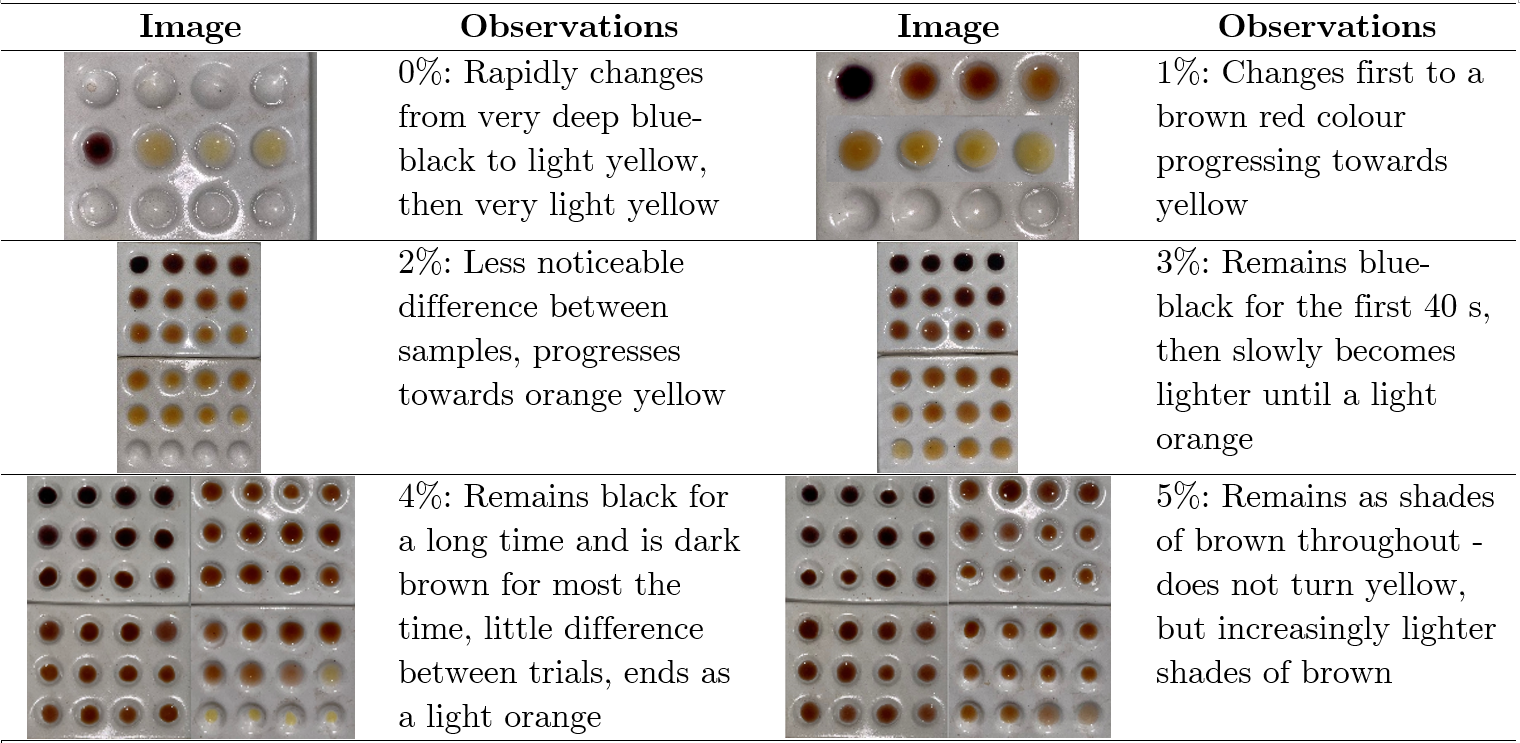
\includegraphics[width=\textwidth]{images/qualtable.png}
    \label{qualitative}
\end{figure}
\end{center}

\vspace{-20mm}

\begin{center}
\begin{table}[H]
\centering
\caption{\label{processed}Processed data showing the lemon water concentrations of 0.0\%, 1.0\%, 2.0\%, 3.0\%, 4.0\% and 5.0\% and amylase rate of reaction ($\frac{mL \text{ consumed}}{s}$) over 5 trials with calculated mean and standard deviation.}
\begin{tabular}{cccccccc}
\rowcolor[HTML]{FFFFFF}
\cellcolor[HTML]{EFEFEF}{\color[HTML]{9B9B9B} } & \multicolumn{5}{c}{\cellcolor[HTML]{FFFFFF}
\begin{tabular}[c]{@{}c@{}}Amylase Rate of Reaction ($ \frac{mL \text{ consumed}}{s} \quad \pm 0.5$) \end{tabular}} & \cellcolor[HTML]{EFEFEF} & \cellcolor[HTML]{EFEFEF} \\
\rowcolor[HTML]{EFEFEF} \begin{tabular}[c]{@{}c@{}}Concentration of \\ Lemon Water \\ (\% $\pm 0.05$) \end{tabular} & Trial 1           & Trial 2           & Trial 3           & Trial 4           & Trial 5           & \begin{tabular}[c]{@{}c@{}}Mean Rate \\ of Reaction \\ ($\frac{mL}{s} \pm 0.5$) \end{tabular}  & \begin{tabular}[c]{@{}c@{}} Standard \\ Deviation \end{tabular} \\
0.00        & 2.5                & 2.5                & 2.5                & 2.5                & 1.7                & 2.3        & 0.37 \\
\rowcolor[HTML]{EFEFEF}
1.00        & 0.42                & 0.42               & 0.39                & 0.42                & 0.36                & 0.40        & 0.027 \\ 
2.00        & 0.13              & 0.14               & 0.13               & 0.14               & 0.13               & 0.14       & 0.0040 \\
\rowcolor[HTML]{EFEFEF}
3.00        & 0.10              & 0.11               & 0.11               & 0.10               & 0.10               & 0.10       & 0.0040 \\
4.00        & 0.060               & 0.061               & 0.060               & 0.061               & 0.061               & 0.060       & 0.00073\\
\rowcolor[HTML]{EFEFEF}
5.00        & 0.052               & 0.051               & 0.053               & 0.052               & 0.052               & 0.052       & 0.0010 \\ 
\end{tabular}
\end{table}
\end{center}

\vspace{-15mm}

The rate of reaction was calculated by dividing the volume of the substrate consumed, which was 2.5 mL starch in every reaction, by the time taken for consumption as shown below:

\vspace{-5mm}

\begin{equation}\label{samp.2}
    \frac{2.5 \text{ mL}}{10 \text{ s}} = 2.5 \frac{\text{mL}}{\text{s}}
\end{equation}

The mean was calculated by taking the sum of all the calculated rates of reactions of the trials within one concentration, and dividing it by the total number of trials, 5, with the sample calculation \ref{samp.1}. Standard deviation was calculated with Excel's standard deviation function, =STDEV.S, where all the trials in a concentration where inputted into the calculation.

\begin{equation}\label{samp.1}
    \frac{2.5+2.5+2.5+2.5+1.7}{5} = 245
\end{equation}


\begin{figure}[h]
    \centering
    \caption{Processed data graph showing mean amylase rate of reaction against the lemon water concentrations (0.0\%, 1.0\%, 2.0\%, 3.0\%, 4.0\% and 5.0\%) with error bars showing standard deviation.}
    \label{fig:graphh}
    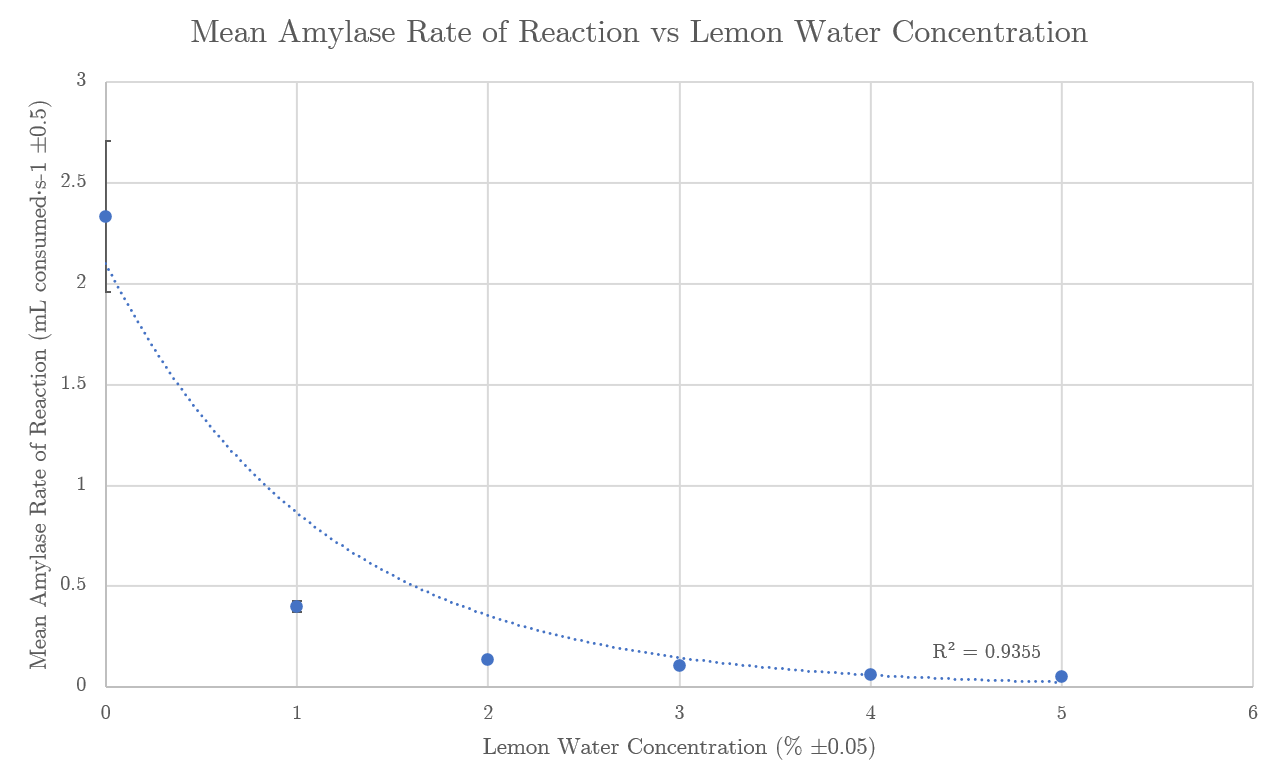
\includegraphics[width=0.59\textwidth]{images/graph.png}
\end{figure}

The relationship between the rate of amylase reaction and an increasing concentration of lemon in water shows a strong negative exponential relationship. As seen in Figure \ref{fig:graphh}, the reaction rate of amylase, as demonstrated by the time taken for Lugol's Iodine to change colour (indicating the complete consumption of the starch), decreases in an exponential manner relative to the increase in lemon juice concentration.

The coefficient of determination, a Spearman's rank correlation and the error bars indicate a strong statistical significance of these results. Since the data is not linear but presents a negative trend, Spearman's rank correlation is an appropriate test that assesses how well the relationship between the variables fits a monotonic function (\citeauthor{lund_lund}). Spearman's $\rho$ was calculated by plotting the lemon water concentrations against the mean rates of reaction in an online calculator provided by Social Science \citeauthor{social_science_statistics}, showing a value of $\rho = -1$, indicating a statistically significant association to a negative monotonic function - fitting the model of the exponential function in Figure \ref{fig:graphh}. Furthermore, the high coefficient of determination value, $R^2 = 0.9355$ (Figure \ref{fig:graphh}), indicates a strong  relationship between the data and the plotted regression. The error bars also do not overlap, indicating that the difference between each of the means recorded is statistically significant. However, it is important to note that the first value at 0\% concentration has a large standard deviation, however, since the regression function falls within this standard deviation, it represents the data accurately.

The qualitative data supports this trend as can be seen in the spotting tiles in Figure \ref{qualitative}. As the lemon juice concentration increases from 0.0\% to 5.0\%, the time taken (where each well represents 10 seconds) for the amylase to completely hydrolyse the starch increases as the overall colour of the solution changes less rapidly (where more wells have the same colour), supporting the inverse relationship between lemon juice concentration and amylase activity. 

It is interesting to note that the trend shown in Figure \ref{processed} approaches an asymptote of 0 amylase activity. This supports the idea that as the pH strays further from the optimal pH of 7.0 and becomes more extreme, it can denature the enzyme by breaking the bonds in the quaternary and tertiary structures, thus causing it to lose its function. As a result, for higher lemon juice concentrations, the acidity may denature the amylase resulting in an immediate fall to 0 enzyme activity, which is demonstrated by the trend. 

\section{Evaluation and Conclusion}

\subsection{Conclusion}

This experiment investigated how an increasing concentration of lemon juice in a water solution affects the enzymatic activity of $\alpha$-amylase. The data supports the hypothesis which predicted an inverse relationship between the rate of reaction and concentration increase, where, by finding the average rate for amylase to consume the starch using the time taken for Lugol's Iodine to indicate a lack of starch presence with the increasing concentrations, a negative exponential relationship was established between the variables that was equally supported by the qualitative evidence. These conclusions align with Oboh et al.'s experiment, which investigated the inhibition of amylase specifically from citrus extracts, and found that lemon peels had a greater inhibitory effect than orange peels due to their lower pH (\citeauthor{oboh_olasehinde_ademosun_2017}). Further research demonstrated how meals consumed with beverages of low pHs, with lemon juice in particular having the most significant effect, result in a slower starch digestion as measured by capillary blood glucose concentrations (\citeauthor{freitas_le_feunteun_2019}). Both these studies corroborate the link found between a decreased pH, specifically from the addition of lemon, and amylase inhibition demonstrated by the decreased rate of reaction in this investigation. 

\subsection{Strengths and Limitations}

Certain aspects of the design of the experiment and reliability of the results were strengths in this investigation. The selected range of independent variables accurately represented the concentrations of lemon water matching the context of the investigation and provided reasonable grounds for the investigation in which the amylase was able to hydrolyse the starch completely. Furthermore, the external factors that could potentially affect the results of the experiment were controlled very well, where temperature and concentration, the other two factors that influence rate of reaction, were controlled by using a water bath and measuring each concentration in a graduated cylinder ($\pm 0.5$) respectively. As a result, the results had a relatively low standard deviation, indicating a small range of data and thus reliable results. 

The method of measuring the starch concentration in wells with a time interval was a great limitation. Although 10 s time intervals were the fastest this experiment could be reasonably and accurately conducted, the very large uncertainty of $\pm 5$ s allowed for a lot of data to be lost, particularly in the lower concentration trials such as the 0\% as the actual time for reaction was not known, simply that it was less than 10 s in most situations. As a result, this could've disproportionately changed the reaction times, especially for the lower concentrations. To mitigate this effect, multiple people can be involved in the experiment to improve the efficiency of measuring the starch concentrations, decreasing the time delay between measurements.

Furthermore, the reliance on qualitative observations to determine the point at which all the starch was hydrolysed was not reliable. The appearance of the final Lugol's Iodine colour varied slightly between trials, ranging from light orange to light yellow, indicating there were slight differences in the final starch concentrations. However, this is an expected flaw when using a qualitative method. This could've affected the data in either direction: the time taken could be overestimated, where a yellow colour was not considered as completely hydrolysed whereas in another trial it was, or also underestimated, where a slightly darker colour was decided to be the endpoint of the reaction when in fact the amylase could've hydrolysed more starch. To improve this, a colour reference can be used to ensure the reaction is only deemed as complete when Lugol's Iodine reaches a specific colour that can be maintained consistent across trials.

\subsection{Extensions}

While this experimented supported the conclusion that drinking lemon water can inhibit amylase by reducing its rate of reaction, the actual implications of salivary amylase inhibition on digestion could be further investigated. Since amylase is also secreted by the pancreas leading to starch digestion in the small intestine, the significance of this initial inhibition can be explored in the context of digestion as an entire process. In addition, not only the impact of different beverages, for example, tea or coffee, but also temperature of the beverage on amylase inhibition can also be explored to further understand the conditions under which salivary amylase is inhibited. 


\pagebreak

\printbibliography

\end{document}